\documentclass[12pt, a4paper,oneside]{report}
\usepackage{titlesec}
\usepackage[utf8]{inputenc}
\usepackage[T1]{fontenc}
\usepackage{textcomp}
\usepackage{framed}
\usepackage{pbox}
\usepackage{caption}
\usepackage[nottoc,numbib]{tocbibind}
\usepackage[pdftex]{graphicx}
\usepackage[toc]{glossaries}
\usepackage{amssymb, amsmath}
\usepackage[colorlinks,
pdfstartview = FitH,
linkcolor = black,
plainpages = false,
hypertexnames = false,
citecolor = black]{hyperref}
\usepackage{setspace}
\setstretch{1.25}
\usepackage[left=3.5cm,right=3.5cm,top=2cm,bottom=2cm]{geometry}
\graphicspath{{./pics/}}
\usepackage[printonlyused]{acronym}
\usepackage{todonotes}
\usepackage{subcaption}
\usepackage{float}
\usepackage{pifont}
\newcommand{\cmark}{\ding{51}}%
\newcommand{\xmark}{\ding{55}}%
\usepackage{multirow}
\usepackage{pdflscape}
\usepackage{eurosym}
\usepackage{tocbibind}
\usepackage[english]{babel}
\usepackage[utf8]{inputenc}
\usepackage{multirow}
\usepackage{subcaption}
\usepackage[section]{placeins}
\usepackage{lscape}
\usepackage{adjustbox}
\usepackage{graphicx}
\usepackage{amsmath}
\usepackage{algorithm}
\usepackage{booktabs}
\usepackage{tabularx}
\usepackage{placeins}
\begin{document}

\begin{titlepage}
	Universität Passau\newline
	Fakultät für Informatik und Mathematik
	\vspace{2.5cm}
    \begin{center}
    \LARGE\textbf{{Classification  Of Visualization  In Scientific Literature}}\\
   
    \normalsize

    \vspace{2.5cm}
    \end{center}

 \normalsize{
 	Masterarbeit zur Erlangung des akademischen Grades\newline
 	Master of Science (M.Sc.)\newline
 	\ \\
 	Lehrstuhl für Intelligent Systems und Lehrstuhl für Data Science \newline
 	der Fakultät für Informatik und Mathematik\newline
 	der Universität Passau\newline
 	
 
    \begin{tabular}{ll}
    	Name: & Arnold Azeem \\
    	Matrikelnummer: & 79176 \\
    	Fachbereich: & Informatik\\
    	Studiengang: & Master Informatik\\
	Erstprüfer: & Prof. Dr. Christin Siefert \\
	Zweitprüfer: & Prof. Dr. Michael Granitzer\\
	Date: &     \today
    \end{tabular}\\
    }



\newpage
\begin{abstract}
Distinct visualisation techniques are used in scientific research publications to summarise large amount of data and also represent a variety of data. These visualisations help to communicate complex information and support the arguments being presented in the publication in a way that is easy to understand and follow.
These figures tend to reveal trends, patterns or relations that might have otherwise been difficult to grasp using only text. 
It is therefore relevant that we extract the data from these visualisations since the extracted data can be used for validating the publication or presenting the data in another form for a different audience. In this context, classifying these visualisations is the initial step since, there is a variety of visualisations and each one is processed in a specific way. It is only after classification that extraction of raw data from these visualisations can be acquired for other tasks. This thesis presents an approach whereby real world data is used to create four types of plots (scatter plots, bar charts, line charts, and box-plots) and random plots also of the same kind from the Internet are added together and used to train and evaluate a CovNet model to be able to classify these plots. 
\end{abstract}

\renewcommand{\abstractname}{Acknowledgements}

\end{titlepage}
\setcounter{tocdepth}{10}

\clearpage
\tableofcontents


% \begin{acronym}

% \acro{XML} {Extensible Markup Language}s

% \end{acronym}

\listoffigures
\listoftables

\titleformat{\chapter}{\LARGE\bfseries}{\thechapter}{1em}{}

\newpage


\newpage
\chapter{Introduction}
``The human brain processes images 60,000 times faster than text, and 90 percent of information transmitted to the brain is visual'' \cite{humaneye}. This buttresses the fact that information and data is easily understood when visualised, for this reason most scientific publications tend to present their data using tables, plots and pictures. Identification, extraction and interpretation of this visualised data for purposes of validation of results by another researcher, or presentation of the data to another audience is an area in machine learning which is still found wanting.\newline\newline
The aim of this thesis is to develop a reliable system for the purpose of recognising chart images by using example chart images created with real world data. Image processing and machine learning methods are the main constituents of this thesis. The initial section in this chapter gives an overview of chart image classification and the complications and difficulties faced in chart image classification.  The other parts of this paper are organised in the follows: 
In the other sections of this chapter the research motivation, objectives, contributions and an outline of
the proposed framework in this thesis is presented. Finally, the structure of the rest of this thesis is illustrated in Section 1.6

\section{Overview} 
A basic description of a chart is a graphical representation of data, where the data is represented by some type of symbols. These symbols could be rectangles in the case of histograms or bar charts,  slices that make a circle in the case of a pie chart, and dots,stars,diamonds and an asterisk in the case of a scatter plot.
Charts are often used to visualise complex data for easy understanding and interpretation, to find patterns and trends in data. Charts can usually be read more quickly than textual data, they are used in almost every field especially in science, marketing, and maths. Charts are mostly created with the help of a computer but can also be created by hand. There are a variety of charts and therefore, to present your data in the right way, the right type of chart must be employed. For example bar charts are best used when comparing data, line charts works better when we want to find trends in data and scatter plots are used when we want to find relationships in data. Figure \ref{fig:chartse} which was inspired by the figure from \cite{chartselection} shows which charts we should choose depending on what we would like to describe in some acquired data. For example if we want to show a relationship between two variables in some data, we should a scatter plot as seen in the figure.\\

\begin{figure}[!htb]
	\centering
	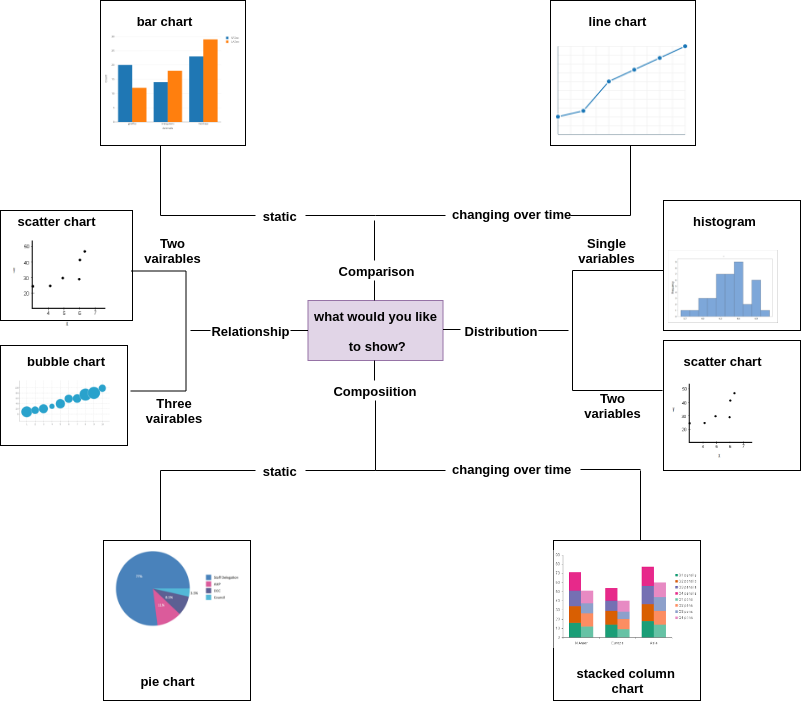
\includegraphics [scale=0.5] {chart}
	\captionof{figure}{Seletecting the approapriate chart for visualising data }
	\label{fig:chartse}
\end{figure}

Charts usually appear in different forms, nonetheless there are some features that are mostly present in every chart. Charts are mostly graphical with a little bit of text used to annotate the data. One important use of text visible in most charts is to give the chart a title. The title describes what the graphic represents and is usually situated above the main graphical part. Text is used less because the brain processes visual information sixty thousand faster \cite{humaneye} as mentioned earlier. Most graphs have one line at the side and another usually at the bottom. These lines if used are called axes of the graph. The one at the bottom is called the x-axis, and the other line the y-axis. Each graph usually indicates numerical or periodic sequence shown by periodic graduations. The are also texts usually outside or besides the axis describing the measurements.
Some charts include what we call a legend, the legend is usually present in situations where there are multiple variables to be described. Figure \ref{fig:boxy} shows a typical chart that has the features mentioned above. The legend showing the two variables female and male represented in the chart, the label on the left side annotating the cholesterol levels with the different measurements of the cholesterol shown on the y-axis, and to the bottom categorical measurements shown on the x-axis. Finally the title, that is the text describing the whole chart shown at the top. 

\begin{figure}[!htb]
	\centering
	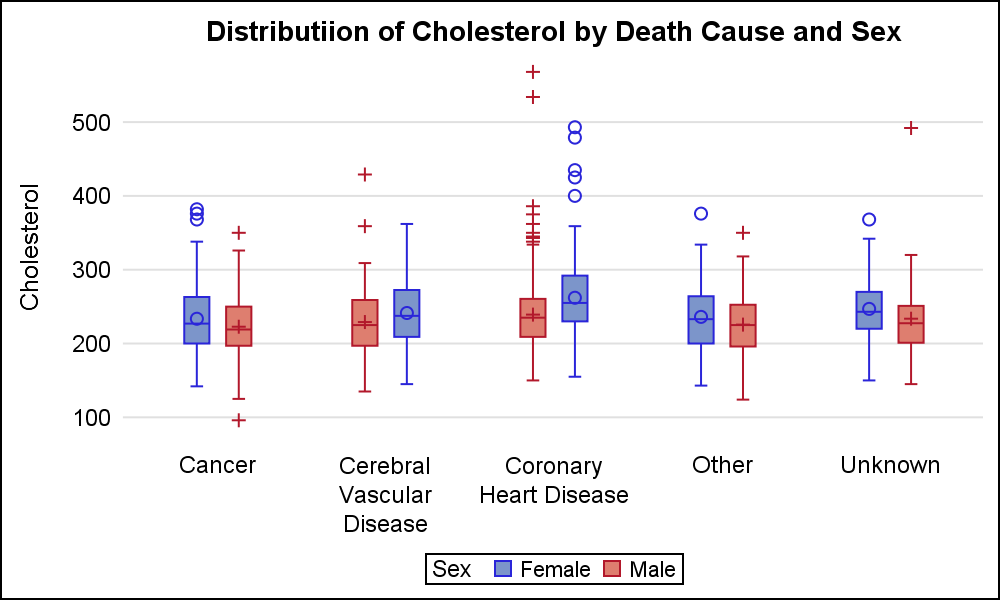
\includegraphics [scale=1.0] {box_color.png}
	\captionof{figure}{A box plot with a legend, x-axis, and y-axis from \cite{boxy} }
	\label{fig:boxy}
\end{figure}

Despite most features being present in most charts, there are some charts that are totally different from the rest. For example a pie chart does not have an x-axis or y-axis, also the designers of a particular chart have a choice of visual encoding and styling, this results in a wide variety of charts, even in charts of the same type. To be able to identify the different types of charts will mean having all the wide range of the different visual encodings and styles of these charts.


\section{Motivation}
Complex data is better explained in scientific documents with the aid of visualisations. These charts present complex data in an easy to understand format as compared to the textual content. 
Chart images are an important part of scientific documents.
Data is ever growing and sometimes complex, and therefore using figures and diagrams to interpret and represent this data cannot be undermined. Chart images provide a way to easily give insight to  research findings, which would have otherwise been more complex relying on only textual data. The data which these visualisations contain when extracted play an important role in events where another researcher wants to verify the work of the publisher. The extracted data can also be used to develop other visualisations in situations where the paper needs to be presented to a different audience with a distinct background as opposed to the audience for which the visualisations were created initially. Another reason for extracting this data is that, when comparing two plots, looking at the raw data, gives us more insight and consequently helps in better decision making as compared to just looking at the figures. Since each plot will be processed differently to extract the raw data, it is relevant that we can distinguish one plot from another. For this reason, there has been a growing interest in the chart analysis area and quite a number of techniques have been developed. In spite of this growing interest, there has been little groundbreaking results achieved due to different variations in appearance of plots \cite{liu2015chart}. For example, Manollis Savva, et a \cite{savva2011revision} proposed a model to classify charts using extracted low-level features and textual features. After extracting the features, a  Support Vector Machines (SVMs) classifier is used for the classification step. This method was limited since most charts contain the same type of features like axes, grid lines, and legends. In V. Shiv Naga Prasad's work \cite{prasad2007classifying} classification was based on using features based on the shape and spatial relationships of their primitives. This work was limited due to the inconstancy in which data in most charts can be depicted. However in the paper of Alex Krizhevsky et al.~\cite{krizhevsky2012imagenet} a deep CovNet which combines both feature extraction and classification was used and this technique achieved good results.

\section{Objective}
The aim of this thesis is to develop algorithms using image processing and machine learning methods for the purpose of chart image classification. Different approaches will be considered in other to choose the most favorable one.\\
The goal of this thesis is to try to identify or recognise chart images with the highest accuracy. To achieve this goal we have to answer the question: \begin{quote} How Well Can We Classify the Four Different Types of Plots (Line-Charts, Bar-Charts, Scatter-plots, and Box-plots) in Scientific Literature? \end{quote} 
To answer this question, the following objectives are set.

\begin{itemize}\itemsep3pt
	\item obtain raw data gathered from real world occurrences.
	\item create a dataset of chart images with the collected data. Using  different plotting programs (Python, Matlab, R, and Java) and different libraries supported by these plotting programs.
	\item train and evaluate a machine learning model that can recognise unseen charts with high accuracy. The four classes of plots are box plots, line charts, scatter plots and, bar-charts.
\end{itemize}

\section{Research Significance and Contribution}
Figure \ref{fig:vis} shows the significance of this work and what it will lead to. This thesis focuses mainly on four chart images. These plots are scatter-plots, bar-charts, line-charts because they are 3 of the most popular image charts and box-plots because it shows skewness and unusual observations in a dataset and this information is especially relevant when dealing with large data, which is mostly the case in machine learning. The first part of the diagram involves, obtaining  the four different types of plots mentioned earlier, after which we then label our plots and train a neural network model to be able to classify with high accuracy any of the four plots if shown to our model, then finally the raw data can be extracted from the detected plot using other processes and techniques. The focus of this thesis however, is shown in the figure with red dotted lines, which entails, gathering a dataset of chart images, labeling them, training the model and classifying the plots. \\

\begin{figure}[!htb]
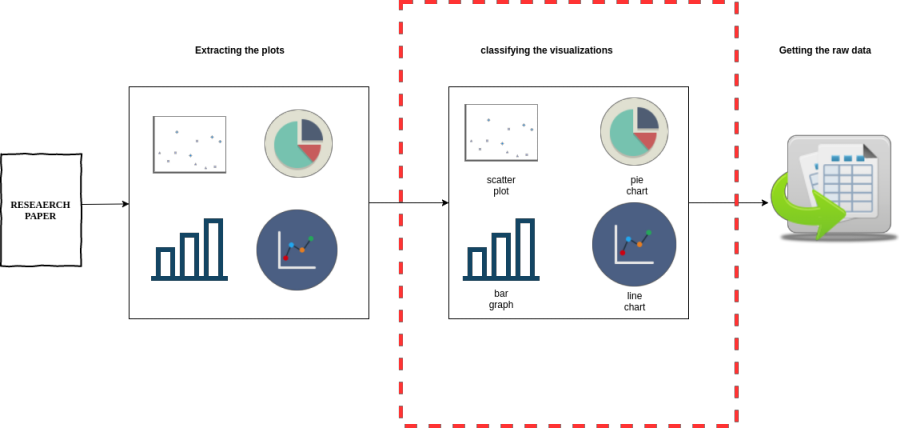
\includegraphics [scale=0.48] {vision}
\captionof{figure}{Overview of process to obtain raw 
	data from scientific papers. The red outline indicates the work in this 
	thesis.}
\label{fig:vis}
\end{figure}


\chapter{Background and Related Work}



\section{Overview}
In this chapter the literature on classification of chart images is presented and explored. Old techniques that were previously used and how they evolved are discussed. Section 3.2 introduces the two main categories images classification has been put into, while in 3.3 and 3.4 these two categories are discussed in detail, also, CovNets which are inspired by the cat’s visual cortex and have performed really well in the field of image processing are talked about in detail. Lastly, Section 3.5 presents the important approaches and techniques employed by other researchers for chart image classification.


\section{Background}
Classification involving charts images has been a topic of huge interest in recent times. This is due to the fact that, most scientific publications if not all, are embedded with these charts as a way of conveying complex research findings in more visualisable and easy to understand format. As a result of this popularity chart images have gained, different techniques have over time been used for classification of charts and these techniques have evolved over the years. The techniques have been inspired by techniques from image processing, raster to vector conversion and layout analysis. These techniques can be put into two categories, Model-Based Approaches and Machine Learning Based Approaches ~\cite{amara2017convolutional}. In the next section, the methods and techniques used in this thesis, and techniques that inspired us to choose these techniques are explained in details.

\section{Model Based Approaches}
The following is written with inspiration from Boyle et al. work~\cite{boyle2007advances}. Numerous chart images even of the same type, are different in sense of their context structure. This is as a result of the variability of positions of the context structure of a chart. There is exists no real standard for all charts to follow, content like; legends, axes, grids etc., have no fixed positions and sometimes are not even present in some charts. As a result of this non standardisation of charts, classifying becomes a difficult task. As a results this approach tries to uses the structure of the charts. The model-based approach is divided into two steps. Firstly, a number of predefined object classes are created with abstract models and then an image is matched with the created model. For example, a model for a 2D/3D pie chart consists of line segments (radii and circular/elliptical arcs), and these line segments are used to create the model, however, just using these line segments wont be enough, so some constraints are introduced into the model, example of constraints of a pie chart include; the center of the pie chart is where all radii meet; all 2D pie charts have radii of equal length; arcs mainly form parts of the same 2D pie chart circle, or if its a 3D then the arcs form part of the ellipse. After this a goodness-of-fit is introduced to help measure the discrepancy between the image and the conditions for the model. For example, a goodness-of-fit of a pie chart is as follows: difference in length of radii; difference in how the arcs are curved; distance between a center of a circle and that of a radii. When a chart is presented for classification, the edges are detected, thinned, linked, vectorised, extracted and compared to the various edge models created and the best match is selected. After this, the good-to-fit criteria is used to measure the difference between the edges of the model and the image. Finally, a voting is performed base on the value of the good-to-fit results. The model-based approach has some drawbacks though. The main drawback is that human intervention is needed to develop the various models. This could be a cumbersome and time consuming procedure. Due to the limitation of this approach a machine learning approach was introduced to handle some of the limited of this approach.


\section{Machine Learning Based Approaches}
This method was developed in recent times, and most works in area of text mining and image processing employ this approach. This method 
involves using handcrafted features extracted from the charts for classification task. In Zhou and Tan's ~\cite{zhou2000bar} work, features like legend, x-y-axis title, chart title, and values of the bar of a bar-chart were extracted for purposes of classifying a bar-chart. In Shao and  Futrelle's~\cite{shao2005recognition} work, graphical elements of the charts like colors,tick marks on an axis and data point markers are the handcrafted feature used for classification. Another instance where handcrafted features were used was in Inokuchi et al. work~\cite{inokuchi2000apriori}. In this work regularly appearing substructures of chart are extracted and used as features for classification. After the feature acquisition step, the obtained features are then represented in vector form for the classification step. The features are stored in a matrix vector-like structure. Algorithm~\ref{alg:1} shows an example of the structure in which the features are stored. This structure has multiple columns containing the features and one column indicating the target or label of the chart. This vector-like structure is then fed as input into a machine learning technique for the model training step. In Karthikeyani and Nagarajan's paper~\cite{karthikeyani2012machine} after the features were obtained SVM Classification \footnote{http://www.statsoft.com/Textbook/Support-Vector-Machines}, MLP Classification
\footnote{http://www.iro.umontreal.ca/~bengioy/ift6266/H12/html/mlp\_en.html}, and  KNN Classification\footnote{
https://kevinzakka.github.io/2016/07/13/k-nearest-neighbor/} were used to create a function that maps the set of features to a predefined label. This technique achieves good results but, the drawback is the over reliance on handcrafted features. This drawback makes it difficult when large amount of data consisting of a variable context structure is involved, and this situation is evident in most cases. Recently, however CovNets (this abbreviation stands for Convolutional Neural Networks and will be used a lot through this work) \footnote{https://deeplearning4j.org/convolutionalnetwork}, a machine learning technique which removes the drawback of using handcrafted features by learning important features anywhere in the image by itself. CovNets performance on image classification keeps on improving and in recent times, results are being compared to human performance levels. CovNets were used in this work, in the next section they will be explained into details, and is inspired by an article written by Daphne Cornelisse \cite{covnet}.\newline

\subsection{The Brain}
The following is . As human beings we identify objects around as all the time with minimal effort. We identify objects based on what we previously leaned. We see objects, label, recognise patterns, and make predictions subconsciously everyday. How are we able to do this effortlessly? Even though the whole process starts with the eye, most of the process happens in the part of the brain called the primary visual cortex. When we see an object, light receptors send signals via the optic nerves to the visual cortex and sense is made of the perceived object by this organ. The deep neural connections in the brain plays a major role in remembering and identifying objects.

\subsection{Input data format}
This section was inspired by Nikhil B's article \cite{input}. Just like the way the human eye needs to perform some preprocessing steps before an image signal reaches the brain, an image recognition system can better identify images if some preprocessing steps were performed on the input images. Below some effective preprocessing steps that go a long way to improve image recognition are explained:

\begin{itemize}
	
	\item \textbf{Uniform aspect ratio:}  Neural networks usually take as input square shaped images, all images should consequently have the same size and aspect ratio. Images should for this reason be checked and cropped to meet this requirement appropriately. One important thing we should consider when cropping is to keep the middle part as much as possible.
	
	\item \textbf{Normalising image inputs:} This step is mainly performed to ensure that there is uniform distribution in the image pixels data distribution.This in the long run accelerates convergence during the process of training. 

	\item \textbf{Dimensionality reduction:} Depending on the type of experiment being performed, the RGB channels of a colored image can be collapsed and convected to a gray-scale channel. This can result in a faster training time.
	
	\item \textbf{Data augmentation:} This step is also dependent on the type of experiment being done. Variant of the input image are acquired by argumenting the existing dataset. This includes scaling, rotation etc.
		
\end{itemize} 



\subsection{Convolutional Neural Network}
Just like how human beings learn to recognise and label objects, we need to show an algorithm a huge number of images for it to be able to identify an image it has never seen before. Computers unlike humans perceive images as a 2D array of numbers, known as pixels. A CovNet has neurons just like the visual cortex and these are organised into layers. Each layer tries to identify a part of the input image. For example on layer identifies the edges, another identifies the curves and so on. This is done by employing the spatial relation that exit in the pixel of an image. All the layers are connected to each other. There are four main layers in the CovNet:

\begin{itemize}
	\item Convolution
	\item Non Linearity (ReLU)
	\item Pooling or Sub Sampling
	\item Classification (Fully Connected Layer)
\end{itemize} 


\begin{figure}[htb!]
	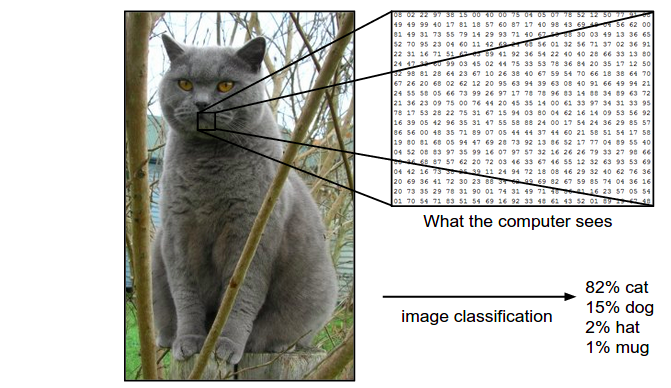
\includegraphics [scale=0.5] {cat}
	\captionof{figure}{How a computer perceives an image- source \cite{softmax}}
	\label{fig:cat}
\end{figure}



\subsection{Convolutional Layer}
The Convolutional layer will be explained using the following example, let consider the image as a magical cake of height and width 48x48, and there is a cake cutter of size say 5x5. The cutter is used to cut the cake from the top left. The cutter is referred to as a filter in machine learning. The cutter in this case is also an array of numbers called weights and for the maths to work the cutter must have the same depth as our cake (5x5x3).
Lets first consider the cutter being in the first position ie. the top left of the cake. The values in the cutter are multiplied with the values of the cake (element wise multiplications). These multiplications are all summed up and result in a single number. This single number is only for the first part and this process is repeated through out the whole cake (Next step would be moving the cutter to the right by 1 unit, then to the right again by 1, and so on) keep in mind its a magical cake so you can cut a part more than once. After using the cutter on the whole of the magical cake we result in a new cake of size 28x28x1, the results is called a feature map. The filters are low level feature identifiers (straight edges, simple colors, and curves). 


\subsection{Activation Functions}
The activation functions are a important part of a CovNet, they are mostly added to the output end of a Convolutional layer. It usually maps the output values between 0 and 1 or -1 and 1. The activation functions can be divided into two categories; linear and non-linear functions. The non-linear functions are the most used because most of real world data are non-linear. There 3 main types of this function that are mostly used. They are the sigmoid, tanh and ReLu. The sigmoid map the output value between 0 and 1, the tanh maps the output between -1 and 1 and finally the ReLu the most used activation function. The Rectified Linear Units (ReLU) is found in all layers during the Convolution phase, this layer implements element-wise nonlinearity to our Convolutional layer, this just means it helps to handle situations where the relation between the input values and the CovNet output is non-linear. The ReLU has a function \(f(x) = max(0,x)\) which means if you give it a value x, it will return 0 if x is negative and will return the value itself if its positive. We used ReLU mainly because it speeds up the training process significantly and it does not saturate(the gradient is small, if the input is elevated or small) unlike the tanh and sigmoid~\cite{relu}. Figure ~\ref{fig:relu} shows a plot from Krizhevsky et al. \cite{krizhevsky2012imagenet} paper shows that there is a 6x advancement in convergence with the ReLU unit compared to the tanh unit. The bold line represents the ReLU and tanh is the dashed line.

\begin{figure}
	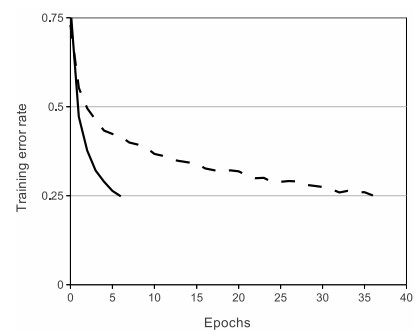
\includegraphics [scale=0.9] {relu}
	\captionof{figure}{ReLU unit compared to the tanh unit from Krizhevsky et al. paper \cite{krizhevsky2012imagenet}}
	\label{fig:relu}
\end{figure}


\subsection{Pooling Layer}
The pooling layers basically have two main functions, first one is that it helps the CovNet to locate features regardless of which part of the image it is located. This results in the model being robust against small changes in position of the features of the images. The second function is that it also helps to reduce the size of the feature map. Therefore computations in the futures layers are relatively less complex. One way of performing pooling is using max pooling technique other less used techniques include Average and sum pooling, the idea in max-pooling is like sliding a window through the feature map, the windows fills a number of arrays in the feature map therefore, you pick the largest among all the numbers and disregard the rest of the numbers. We employ this technique in the first, second and last Convolutional layers of our network.

\subsection{Dropout Layers}
The following is inspired by an article on Medium \cite{dropout}. 
This layer is used for regularising your network. The dropout is used in our CovNet to prevent over-fitting. The Fully connected layers eventually handles more parameters and therefore neurons become co-dependent on one another, and this leads to over-fitting during the training phase. When dropout is implemented in a network, it does not use all neurons during a particular forward or backward pass during training but, chooses random neurons at a specified probability for each pass. Figure \ref{fig:dropout} shows how how a dropout is different from a normal neural network.

\begin{figure}[!htb]
	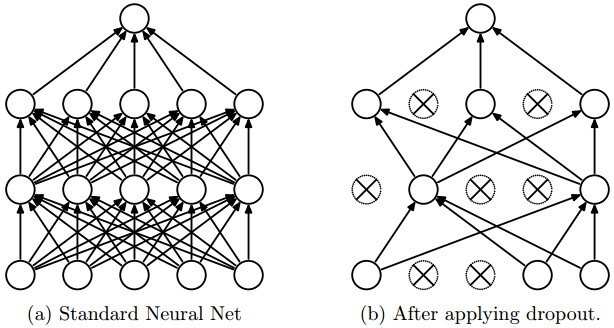
\includegraphics [scale=0.6] {dropout}
	
	\captionof{figure}{Left: shows a standard neural net. Right:
		shows a neural network where dropout has been applied on.
		Crossed units are dropped units. figure from Krizhevsky et al. paper \cite{srivastava2014dropout}}
	\label{fig:dropout}
\end{figure}


\subsection{Fully Connected Layer}
Fully connected simply implies that every neuron from the previous layer is connected to every other neuron in the next layer. The output of this layer are high level features of the image presented to the network. The output of this layer is a probability distribution of all the classes in the network and this is ensured by using an activation function, usually a softmax activation function. We used a sofmax activation as opposed to other activation functions because, it handles low invigoration
in images (say blurry charts) of your neural net with rather uniform distribution and to high invigoration in images (say large numbers, like sharp images) with prediction probabilities between 1 and 0. To put in simple terms, the Convolutional and pooling layers act as feature extractors and the last layer, the fully connected layer act as the classifier.

\begin{equation} \label{eq:soft}
f_j(z) = \frac{e^{z_j}}{\sum_k e^{z_k}}
\end{equation}

The equation \ref{eq:soft} is a softmax function, (z) represents a vector, so the function takes (in z) and crushes it to a probability value between zero and one \cite{softmax}.

\subsection{Image Processing Techniques}
CovNets are very powerful and have the ability to learn features with some level of spatial invariability, this ability however, is limited when it comes to choosing parameters in an efficient manner~\cite{jaderberg2015spatial}. To further improve robustness to spatial invariance test data, some preprocessing techniques like data augmentation are applied on the train data.\\ \\ One relevant feature of CovNet is its multi layer representation, which is responsible for the classification phase. This multi layer representation is not engineered but rather reliant on the data presented to it~\cite{van2017learning}. The multi layer representation determines the kind of features important for the classification task. To find the right multi layer representation, the network must be presented with a variety of instances of the image, so as to be able to capture the different appearance of the image. There are some parts of the image that can be varied and these parts are: the location, the viewpoint, and the size of an object or pattern. We therefore perform some preprocessing techniques in other to capture the 3 main ways images can be altered so that our model is better generalised. 

\begin{itemize}
 	\item Data Augementation: CovNets require a large train dataset in other to learn. The formation of such a dataset is strenuous and expensive task. Data augmenting eases this task by creating label preserving transformations samples by transforming,rotating, flipping or even scaling the original samples. This techniques helps the model to be robust to changes in position and orientation ~\cite{taylor2017improving}. 
 	
 	\begin{figure}[!htb]
 		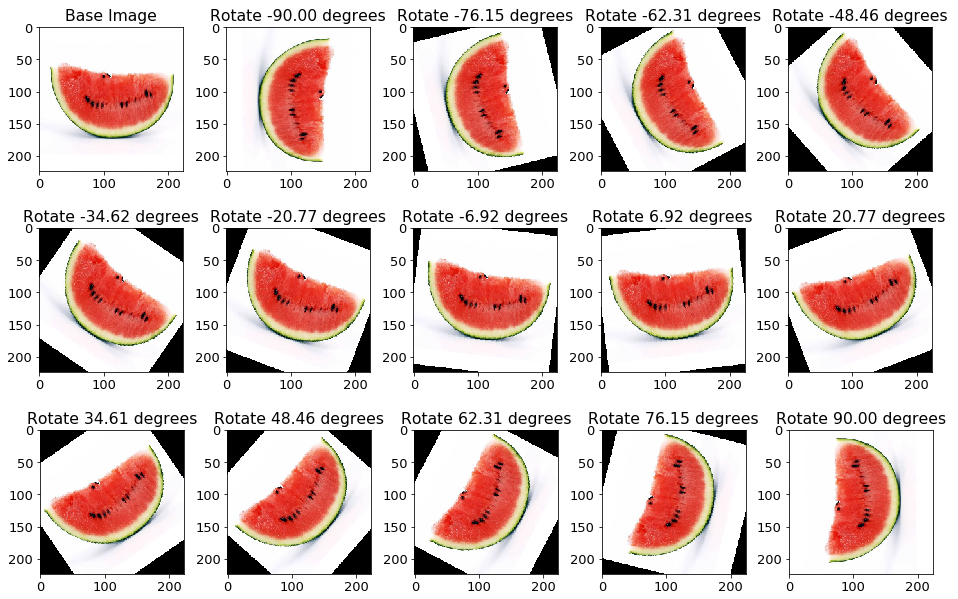
\includegraphics [scale=0.44] {augmentation.png}
 		\captionof{figure}{Data augmentaion technique of Rotation (at finer angles) source \cite{augement}}
 		\label{fig:augment}
 	\end{figure}
 
 \item Normalization: The process where the range of pixel intensity values are changed, this is done to bring the pixels to a range that our senses are more familiar to. The motivation for normalizing image data is to achieve consistency in the range of pixel values in the data. There are mainly two types of normalisation techniques: first one is Scaling, that is putting the values on the same scale and secondly centering, which involves balancing the data around a particular point. Both techniques have different benefits and should be selected based on our needs. For instance scaling speeds up convergence and centering fights the problem of vanishing gradient~\cite{normalizing}.

\end{itemize}

\subsection{Validation in Machine Learning}
Over-fitting is term used in machine learning when a model performs well during training but does badly during the testing phase. 
Lets take a real world example of an athlete, when a runner trains with other runners he is better than without considering the finishing time (parameters), he might think he is the best but this does might be wrong when he partakes in a competition with other runners he had never trained with.


\subsection{Training process}
This section is inspired by a blog written by ujjwalkarn \cite{cnnonline}. The process by which a CovNet performs classification is summarised below.

\begin{itemize}
	\item All parameters (weights, filter, and biases) are initialised randomly.
	\item The network is then given as input the image. The forward pass is then performed (convolution, relu, pooling and fully connected layer),  the output is a probability of each class.
	\item here the error in the output is calculated.
	\[Total Error = \sum  \frac{1}{2} (target probability - output probability) ^2 \]
	\item This step reduces the total error by performing back-propagation, the gradients of the error with respect to the weights are calculated. This is used to update parameters and therefore results in reducing the total error.
	\item In the final step, steps 2 to 4 are repeated for all images in the training dataset. The best parameters are then stored for the prediction of a new image given to the network.\newline 
	
\end{itemize} 

\section{Review of chart image Classification Techniques}
In the rest of this chapter, three related works that performed chart image classification, with unique methods and also achieved good results are described in details.  

\subsection{Machine Learning Classification Algorithms to Recognize Chart Types in Portable Document Format(PDF) Files}
Karthikeyani and Nagarajan's work ~\cite{karthikeyani2012machine} focuses on classifying charts found in pdf files. The steps employed for the classification task involves extracting texture features from the charts and then, using a machine learning technique for the classifying phase. The dataset consists of images extracted from various pdf's. The dataset is made up of 155, 256*256 RGB images in total. Table~\ref{table:pdf} shows the details of the dataset used.
The technique used involved extracting handcrafted features from the chart image and then, using these features as input for a model to be trained and tested.
For the feature extraction phase, Gray Level Co-Occurrence Matrix (GLCM) is employed. GLCM is a technique which uses co-occurrence matrix to extract texture features of an image with the use of statistical equations. GLCM was used to extract eleven features, these included: area, median, minimum and maximum intensity, contrast, homogeneity, energy, entropy, mean, variance, standard deviation and correlation. These extracted features are correlated to the pixels of the image. These extracted features are then stored using a 2-dimensional matrix vector data structure. This structure has thirteen (13) columns and 'x' rows, where x is the size of the dataset. The features are stored in twelve (12) columns and the label is stored in the thirteenth column. The features and labels were stored in the below structure~\ref{alg:1}.

\begin{table}[h]
	\centering \def\arraystretch{1.5} \small
	\begin{tabular}{|p{3cm}|p{3cm}|p{3cm}|p{3cm}|}
		\hline
		Chart Type & No of Charts & Chart
		Type & No of Charts  \\ \hline
		2D Bar chart & 40 & Doughnut 2D & 7 \\ \hline
		3D Bar chart & 16 & Doughnut 3D & 11\\ \hline
		2D Pie chart & 13 & Line & 35 \\ \hline
		3D Pie Chart & 20 & Mixed Chart& 13 \\ \hline
	\end{tabular}
	\caption {Details on Dataset from \cite{karthikeyani2012machine} }	
	\label{table:pdf}
\end{table}


\begin{algorithm}
\caption{This is the structure used to store the features}
\label{alg:1}
Struct FeatureVector \{\\
	float feature1; float feature2;\\
	float feature3; float feature4;\\
	float feature5; float feature6;\\
	float feature7; float feature8;\\
	float feature9; float feature10;\\
	float feature11; float feature12;\\
	int target;\\
\}
\end{algorithm}

This vector like structure is then fed as input into three classifiers SVM, MLP neural network, and K-Nearest Neighbor. These classifiers are then trained and a classification model is formed for the recognition step. After this, to see if the model works well a test set consisting of new records is fed into the model for the model to predict their labels. Three metrics were used to check the performance of the model, these metrics are; error rate,
classification accuracy and speed of classification. The error rates obtained were as followes; MLP 0.30, K-NN 0.22 and SVM 0.23. For the accuracy metrics were as follows; KNN (78.06\%), MLP (69.68\%) and SVM (76.77\%) and finally the speed metric. The speed metric which sum of training and test time results are; MPL was the slowest with 8.38,followed by SVM with 0.31secs and  KNN with 0.26secs. Even though these results were good, the paper proposed extracting features which are related to shape and curves since these features will carry more unique information to distinguish charts.

\subsection{Architecture proposal for data extraction of chart images using Convolutional Neural Network}
Our work is inspired by De Freitas et al.~\cite{junior2017archi}, proposed a way to extract the wealth of information contained in different visualisation techniques. The paper talks about two main stages of accomplishing this task. Firstly, classification of the charts is done since it allows a different variety of chart to be detected automatically allowing the next step, which is the extraction of data from the classified plots. The paper, however, focuses on the first step, classification of charts. In this paper, a Convolutional Neural Network is used for the classification task. The Convolutional neural network encapsulates the characterisation and classification processes during its learning process, unlike other techniques. The dataset used for this task were searched for and downloaded from Google image search. Table \ref{table:rela} shows the chart types which were collected and the number of train and test sets which the respective charts were divided into.

\begin{table}[h]
	\centering \def\arraystretch{1.5} \small
	\begin{tabular}{|p{5cm}|p{3cm}|p{3cm}|}
		
		\hline
		Chart Type & Test & Train \\ \hline
		Area Chart & 50 & 555 \\ \hline
		Bar Chart & 50 & 657 \\ \hline
		Line Chart & 50 & 489 \\ \hline
		Map & 50 & 476 \\ \hline
		Pareto Chart & 50 & 261 \\ \hline	
		Pie Chart & 50 & 361 \\ \hline
		Radar Chart & 50 & 454 \\ \hline
		Scatter Chart & 50 & 552 \\ \hline
		Table & 44 & 236 \\ \hline
		Venn Diagram & 48 & 304 \\ \hline
		Total & 498 & 4345 \\ \hline
		
	\end{tabular}
	\caption {Number of Train and Test Dataset collected}	
	\label{table:rela}
	
\end{table}
For the classification, a variant of CovNet called LeNet-based CovNet model is used. The model was implemented using Tensorflow\footnote{https://www.tensorflow.org/}, LeNet-based CovNet has an architecture which is comprised of 3 convolutional layers, followed by a fully connected layer. The model is trained in a way that the dataset is divided into mini-batches, samples of fixed sizes(100) are selected and fed into the CovNet, as a result of this process the model becomes robust since it learns to generalise from the different min-batches which are fed into the model. Also, all the images are converted to JPG and resized to 224x224x3, that is, 224 pixels of height, 224 of width and 3 layers of output. The other parameters used were 1000 epochs and a learning rate of 0.003. The accuracy at the end of the training process was 70\%.

\subsection{Chart classification by combining deep convolutional networks and deep belief networks}
In another paper by Liu et al.~\cite{liu2015chart}, a new approach was proposed for the process of chart classification. The process involves using CovNet to extract deep hidden features of charts and then deep belief networks then use the extracted features to predict the labels of the charts. Due to a difficulty in acquiring a large number of charts as training data, natural images where first used to train the model and later the model was fined tuned with just over 5,000 collected charts. The types of charts collected were pie charts, scatter charts, line charts, bar charts, and flowcharts. The architecture of the CovNet is made up of five Convolutional layers and two fully-connected layers and then an output layer. The preprocessing steps for the images involve down-sampling them to 256 x 256 x 3, after which each is cropped to a size 227 x 227 from the center and its horizontal flip are extracted as the input of the CovNet, other parameters used for the CovNet include a learning rate that starts with 0.01 initially and is then decreased by a factor of 0.1 after every lOOk iterations, the weight decay parameter was set at 0.0005 and a dropout rate of 0.5. This results in an output of a 5-way softmax which produces the distribution over the 5 class labels and this is used as input for the deep belief network. The deep belief network architecture has three hidden layers, whose dimensions are 5000, 500 and 2000. This results in a softmax predicting the probability
distribution over the 5 categories of charts as output.
The training process was done with 4000 randomly selected images and the rest were used as test set. The accuracy of the model after the evaluation was  75.4\%. Table \ref{table:deep} show the results after the training was done without deep belief networks but pre-trained with the natural images and finally the training done with only the chart dataset but with deep belief networks.

\begin{table}[h]
	\centering \def\arraystretch{1.5} \small
	\begin{tabular}{|p{3cm}|p{3cm}|p{3cm}|p{3cm}|}
		
		\hline
		Chart & CovNets&CovNets+DBN without pre-training & CovNets+DBN \\ \hline
				
		Bar Chart & 75.6\% & 45.6\% & 74.2\% \\ \hline
		Flow Chart & 88.3\%  & 56.8\% & 91.3\%  \\ \hline
		Line Chart  & 71.2\%  & 22.3\% & 67.9\% \\ \hline
	
		Scatter Chart & 69.8\% & 44.5\% & 84.2\% \\ \hline
		Pie Chart & 58.1\%  & 50.1\% & 59.4\%    \\ \hline
		Ave. Accuracy & 72.6\%  & 43.9\% & 75.4\% \\ \hline
		
	\end{tabular}
	\caption {Comparing Results of Proposed Framework from (Liu et al.~\cite{liu2015chart}) }	
	\label{table:deep}
	
\end{table}


\chapter{Approach}
As seen in the previous chapter, different approaches and methods have been described for chart image recognition. Due to the complexity of this task, a CovNet approach is employed for our work. Reasons for selecting this approach include; automatic capturing, learning and extraction of features; parameter sharing which allows the model to learn a single set of weights once, rather than a different set of weights every time~\cite{Rodriguez} and more importantly a performance accuracy nearing human capability. In spite of all the advantages of CovNets, they are computationally expensive to apply on high-resolution images. Fortunately, current GPU capabilities with the help of good optimisation techniques can handle this issue~\cite{krizhevsky2012imagenet}. \newline\newline
The specific contributions of this thesis are as follows: to create a dataset of chart images (scatter-plot, bar-chart,line-chart and box-plot) using real-world data. This chart image dataset tries to capture all variety of structure in the various chart images to be handled. The scripts, libraries, and parameters used in creating the chart images are readily available for the recreation of the dataset. The second contribution of this thesis involves training a CovNet model for recognising these types of chart images.\newline
The rest of this chapter describes into details how the dataset was created, it also describes the CovNet architecture that was used for the classification and evaluation tasks.

\section{Dataset}
The following paragraph is inspired by a blog written on what to look for in training data~\cite{edi}.
The saying 'Garbage in Garbage out' is a valid statement when it comes to creating a dataset for machine learning. The machine learning technique will learn from whatever data fed to it. So if a dataset of good quality is fed into the algorithm, then the model created will also be of good quality. The dataset creation stage is therefore an important stage. In most approaches that worked on chart images classification, the dataset used consisted of chart images downloaded from Google and a few others were obtained from extracting chart images from pdf's. This approach we believe is limited since, we don't know the programming languages, the libraries used and parameters used in creating these charts. This missing information is relevant since it tells us how diverse our resultant dataset is. For example, how are we sure that all the charts that were downloaded from Google, were not only created in Python or Java?, and in such a case how well will a new chart created with Matlab or R be classified. For this reason the dataset comprised of image charts created with different libraries and with dissimilar programming languages. Some random chart images from other works were manually labeled and added to our created dataset. In the next sections, the various datasets and the languages used in plotting are described. To make the dataset as diverse as possible, charts created in each programing language used a different set of CSV files. 

\subsection{Dataset for Matlab}
The Data used for creating the plots in Matlab were randomly chosen from Project Dataset \cite{projectdataset}, a free CSV data repository, DatPlot \cite{datplot} and Plotly CSV repository in github \cite{plotly}. The datasets are multidimensional and compiled from normal day to day activities like dating, what makes people happy etc, and objects like cameras and cars. On the average the datasets used contain about 500 instance and 5 different columns. The biggest dataset is called Speed dating data. It is made up of over 8,000 observations of answers to survey questions about how people rate themselves and how they rate others on several dimensions. The smallest dataset used has 33 instances and 12 columns. It contains information about cars. The number of gears and speed, just to name a few attributes.

\subsection{Dataset for R}
For the plots in R, 13 random CSV files where downloaded from an archive of datasets distributed with R called Rdatasets  \cite{rdata}. Rdatasets is a collection of dataset distributed with R. On the average there are 80 instances and 5 columns in each dataset.
The biggest CSV file is the Australian athletes dataset. It's made of 203 instances and 14 columns and contains attributes like sex,height,weight and sports. The smallest dataset is the Canadian Women's Labour-Force Participation. This dataset has 30 rows and 7 columns. It contains information like average wages of women, percent of adult women in the workforce etc.


\subsection{Dataset for Python}
The data used for creating the plots in Python were 15 randomly seleted csv files also from  Rdatasets \cite{rdata}. The biggest dataset among the 15 is the Monoclonal gammapothy data, it contains natural history patients with monoclonal gammapothy of undetermined significance. The dataset is made up of 1384 observations with 10 columns, it has attributes like age, sex, time of death and last contact in months. On the average each dataset contains about 200 instances and 7 columns of multi-dimensional data. The smallest dataset however contains only 33 instances with 11 columns and is called the Nuclear Power Station Construction Data.The data relate to the construction of 32 light water reactor (LWR) plants constructed in the U.S.A in the late 1960's and early 1970's.

\subsection{Dataset for Java}
For the plots created in java, I used the dataset made available by Plotly \cite{plotly}, a github repository of CSV datasets used in the Plotly API examples. 14 random CSV files were downloaded, the biggest file has 1002 instances and 9 columns, and on the average each file contains about 100 instances and 9 columns. The smallest file however is made of 33 instances and 12 columns called the mtcars file. It contain information about a variety of different car models like the number of gears, speed etc. The table \ref{table:1} contains the names of all CSV files that were used in the different languages with the different plotting programs.


\begin{table}[!htbp]

	\centering
	
\begin{adjustbox}{max width=1.1\textwidth,center}
	
	\begin{tabular}{|p{5cm}|p{3cm}|p{3cm}|p{4cm}|}
		
		 \hline
		 \multicolumn{4}{|c|}{Datasets} \\
		 \hline
				
		Python & Matlab & R  & Java\\ \hline
		
		3d\_line\_sample\_data.csv \par LightFordwardFlapStall.csv  \par line\_3d\_dataset.csv \par
		longley.csv  \par loti.csv  \par lung.csv  \par nuclear.csv  \par timeseries.csv  \par
		USJudgeRatings	\par WVSCulturalMap.csv  \par wind\_rose.csv  \par volcano.csv  \par uspop2.csvm \par tips &
		
		Camera.csv \par Cars.csv \par speedDating.csv \par Cereal.csv  \par happiness.csv \par TestData1.csv \par TestData2.csv  \par mpg.csv \par okcupid-religion.csv  \par spectral.csv
		\par stockdata.csv \par subplots.csv  & 
		
		ais.csv \par Angell.csv  \par Baumann.csv \par Bfox.csv \par cane.csv \par carprice.csv \par Chirot.csv
		Davis.csv \par Ericksen.csv \par Florida.csv \par Highway1.csv \par Pottery.csv \par Prestige.csv 
		salinity.csv \par urine.csv & 
		
		3d-line-plot.csv \par 3d-scatter.csv \par 2011\_flight\_paths.csv \par 2011\_us\_exports.csv \par auto-mpg.csv \par candlestick\_dataset.csv \par finance-charts-apple.csv \par 
		globe\_contours.csv\par hobbs-pearson-trials.csv \par motor\_trend\_tests.csv \par 
		nz\_weather.csv \par volcano.csv \par iris.csv \par mtcars.csv	\\ \hline
		
	\end{tabular}
	
\end{adjustbox}


\caption {Names of datasets used in each plotting program}	
\label{table:1}
\end{table}


\section{Creating Plots}
The motivation for creating a variety of plots to capture all type of plots used in scientific papers was acquired by inspecting the datasets of Architecture proposal for data extraction of chart images using CovNet paper \cite{junior2017archi} and Viziometrics: Analysing visual information in the scientific literature \cite{lee2018viziometrics}. Scripts in various languages were written to handle the plotting and labeling process automatically. All datasets for a particular plot (example scatter plot for python) are put into one folder. The scripts reads each CSV file column by column while creating the plots.
Table \ref{table:paratable} describes how the plots where created in each language. The type column describes the different variety of a particular plot, for example bar charts can be of type stacked, grouped, vertical and horizontal bar charts, also scatter plots types can be a scatter plot consisting of one type of marker, one scatter plot with multiple markers and finally a scatter plot with a line showing the correlation between the plots. 
Figure \ref{fig:bars} shows two different types of bar charts. Figure \ref{fig:bar1} is a stacked bar chart and  Figure \ref{fig:bar2} a normal vertical bar chart.
The Library column shows the different plotting libraries used, the parameter column describes parameters that were changed and finally the number of plots created were also added. The images below the tables are sample images that exist in our dataset of created plots for each language.

	
\begin{table}[!htbp]
	\centering \def\arraystretch{1.5} \small
	\caption {Overview of the varied parameters and libraries used for creating plots in the different plotting programs}	
	\label{table:paratable}
	\begin{adjustbox}{max width=1.1\textwidth,center}
				
	\begin{tabular}{|p{2cm}|p{2cm}|p{3cm}|p{4cm}|} \hline
				
\multirow{10}{*} {\rotatebox{90}{\textbf{Scatter plot}}}  &
		
			Language & Library & Parameters \\ \cline{2-4}
		
	& Python & Matplotlib v2.1.2 \par Plotly v2.5.1 \par Seaborn v0.8.1 & MarkerStyle \par 
	['o', '*', '.', '+','x']  \\  \cline{2-4}	 
		  
	& MATLAB & Default \par Plotly &  MarkerStyle \par ['o', '*','+','x','s']  \\ \cline{2-4} 
		
	& R  & Plotly \par Lattice \par Ggplot2 &  MarkerStyle \par ['o', '*', '+','x','s'] \par geom\_point(shape(1,2,16), size  (3-4)) \\ \cline{2-4}
	
	& JAVA & XChart 3.5.1\par jfreechart 1.0.1 & MarkerSize (15 -18)  \\ \hline
		
	\multirow{10}{*} {\rotatebox{90}{\textbf{Bar charts}}}  & Python & Matplotlib v2.1.2 \par Plotly v2.5.1 \par Seaborn v0.8.1 &   \\  \cline{2-4} 
		
		& MATLAB & Default &  Width of bar(14-16) \\ \cline{2-4} 
		
		& R & Default,Plotly \par R Library \par ggplot2 & space (0-3)  \\ \cline{2-4} 
		
		& JAVA  & XChart 3.5.1 \par jfreechart:1.0.192 \par javafx.scene & PlotOrientation \par (vertical or horizontal) \par with error bars \\ \hline 
			
	\multirow{10}{*} {\rotatebox{90}{\textbf{Line chart}}}	 & Python & Matplotlib v2.1.2 \par Plotly v2.5.1 \par Seaborn v0.8.1 & Linestyle \par ['-', '--', '-.', ':']   \\ \cline{2-4} 
			
		& MATLAB  & Default\par Plotly &  MarkerStyle \par ['o', '*', '.', '+','x','s'] \par markersize [8-10] \\ \cline{2-4} 
			
		& R & Default,Plotly \par R Library \par ggplot2 & \\ \cline{2-4} 
			
		& JAVA & XChart 3.5.1 \par javafx \par JFreeChart & MarkerSize (12-16) \\ \hline
			
	\multirow{9}{*} {\rotatebox [origin=c]{90}{\textbf{Box Plots}}} & Python  & Matplotlib v2.1.2 \par Plotly v2.5.1 \par Seaborn v0.8.1 &  \\ \cline{2-4}  
				
		&  MATLAB   & Default &  \\ \cline{2-4} 
				
		& R & Default,Plotly \par R Library \par ggplot2  &  \\ \cline{2-4} 
		& 	JAVA   & XChart 3.5.1 \par Jfree \par smile & LegendPosition (topleft,topright)  \\ \hline
	\end{tabular}
\end{adjustbox}

\end{table}

\begin{table}[!htbp]
	\centering \def\arraystretch{1.5} \small
	\caption {Overview of the number of plot and different varieties plots in the different plotting programs}	
	\label{table:less}
	\begin{adjustbox}{max width=1.1\textwidth,center}
		\begin{tabular}{|p{3cm}|p{3cm}|p{4cm}|}
			\hline
			\multicolumn{3}{|c|}{Scatter Plots} \\
			\hline
			
			Language & Number of plots  & Type\\ \hline
			
			Python & 1165 &  \multirow{4}{*} {\shortstack { Unique markers, \\ With legends,\\ multiple markers \\ regplot }} \\ \cline{1-2}
			
			Matlab &  1008  &   \\  \cline{1-2}
			
			R  & 1009  &  \\	\cline{1-2}
			
			Java &  1002 &  \\ \hline
			
			\multicolumn{3}{|c|}{Bar Charts} \\	\hline
			
			Language &  Number of plots & Types(bar)  \\ \hline
			
			Python &   1018 &  \multirow{4}{*} {\shortstack {Horizontal and Vertical, \\ Stacked, \\ Grouped bar charts \\ Error bars }} \\ \cline{1-2}	 
			
			Matlab &  1063  &  \\ \cline{1-2}
			
			R &  1022  & \\ \cline{1-2}
			
			Java  &  1143 & \\ \hline
			
			\multicolumn{3}{|c|}{Line Charts} \\
			\hline
			
			Language & Number of plots & Types(Line with)  \\ \hline
			
			Python & 1019 &  \multirow{4}{*} {\shortstack { Markers, \\ Multiple Lines }} \\ \cline{1-2}	 
			
			Matlab   & 1013 &  \\ \cline{1-2}
			
			R &  1132  & \\ \cline{1-2}
			
			Java & 1089 & \\ \hline
			
			\multicolumn{3}{|c|}{Box Plots} \\
			\hline			
			Language & Number of plots & Types(Box with)  \\ \hline
			
			Python  &  1012 &  \multirow{4}{*} {\shortstack { Notches, \\ Multiple Boxes }} \\ \cline{1-2}	 
			
			Matlab   &  1032  &  \\ \cline{1-2}
			
			R & 1113  & \\ \cline{1-2}
			
			Java   & 1036 & \\ \hline
			
		\end{tabular}
		
	\end{adjustbox}
	
\end{table}

\begin{figure}[!htb]
	\begin{subfigure}{.6\textwidth}
		\centering
		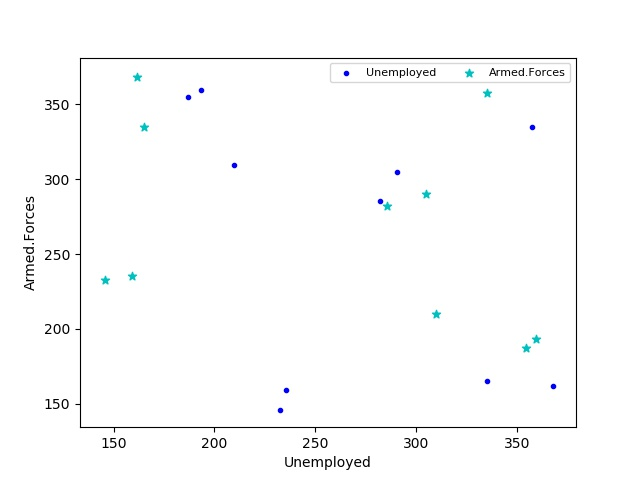
\includegraphics[width=.9\linewidth]{scatter1}
		\caption{Matplotlib scatter plot with star and circular markers }
		\label{fig:scatter1}
	\end{subfigure}%
	\begin{subfigure}{.5\textwidth}
		\centering
		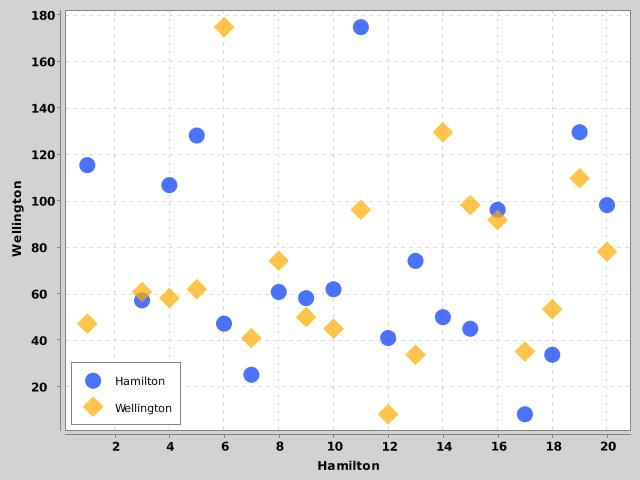
\includegraphics[width=.9\linewidth]{scatter2}
		\caption{Java scatter plot with circular and diamond markers}
		\label{fig:scatter2}
	\end{subfigure}
	\caption{Scatter plots}
	\label{fig:scatters}
\end{figure}


\begin{figure}[!htbp]
	\begin{subfigure}{.5\textwidth}
		\centering
		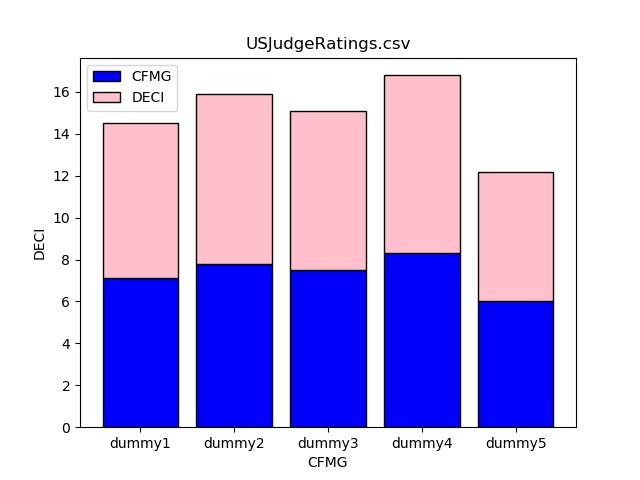
\includegraphics[width=.8\linewidth]{bar1}
		\caption{Matlab stacked bar chart (bar width 16) }
		\label{fig:bar1}
	\end{subfigure}%
	\begin{subfigure}{.5\textwidth}
		\centering
		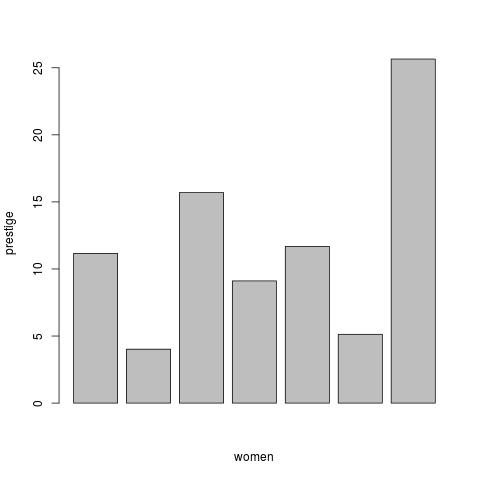
\includegraphics[width=.8\linewidth]{bar2}
		\caption{R horizontal bar chart (bar width 16)}
		\label{fig:bar2}
	\end{subfigure}
	\caption{Example Bar Charts}
	\label{fig:bars}
\end{figure}


\begin{figure}[!htbp]
	\begin{subfigure}{.5\textwidth}
		\centering
		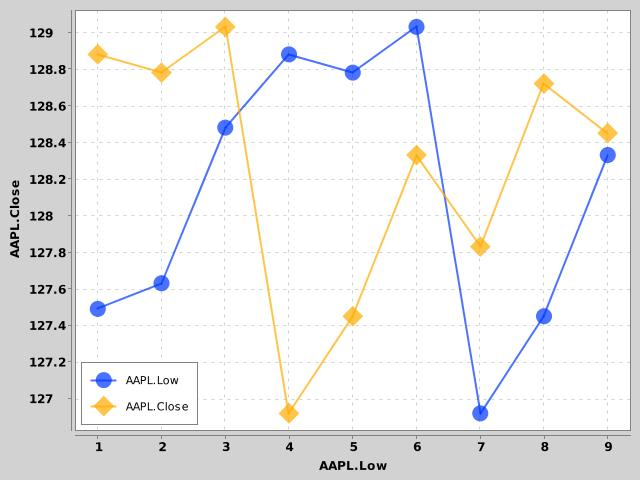
\includegraphics[width=.8\linewidth]{line1}
		\caption{Java line chart with diamond and circular markers }
		\label{fig:line1}
	\end{subfigure}%
	\begin{subfigure}{.5\textwidth}
		\centering
		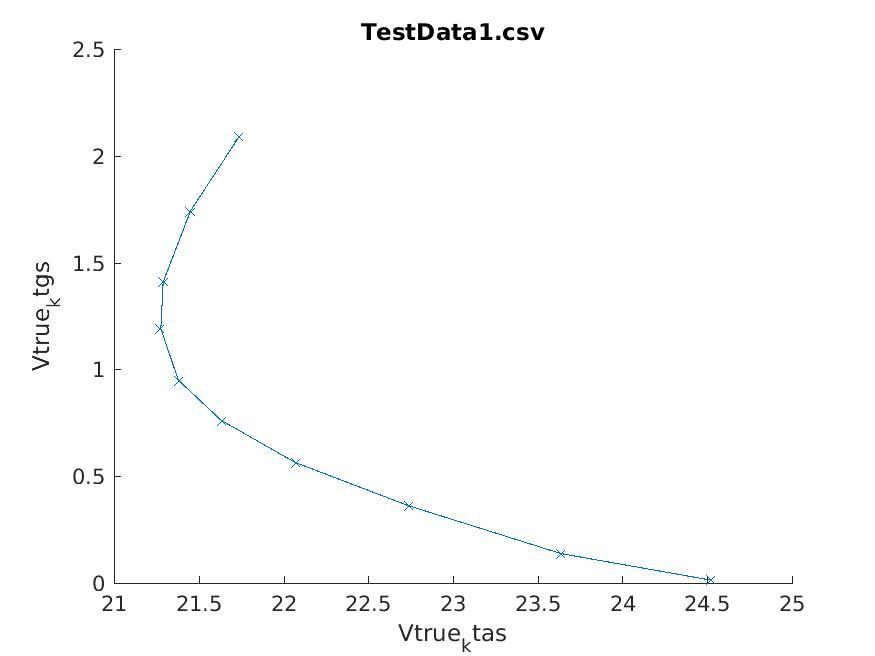
\includegraphics[width=.8\linewidth]{line2}
		\caption{simple Matlab line chart with Asterix marker}
		\label{fig:line2}
	\end{subfigure}
	\caption{Example Line Charts}
	\label{fig:figline}
\end{figure}


\begin{figure}[!htbp]
	\begin{subfigure}{.5\textwidth}
		\centering
		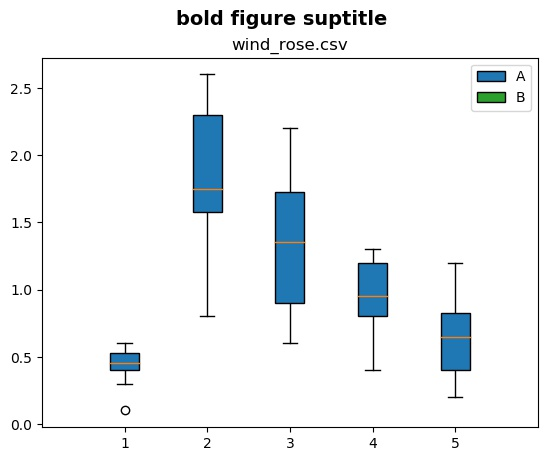
\includegraphics[width=.8\linewidth]{box1}
		\caption{Vertical multiple boxplots in python}
		\label{fig:box1}
	\end{subfigure}%
	\begin{subfigure}{.5\textwidth}
		\centering
		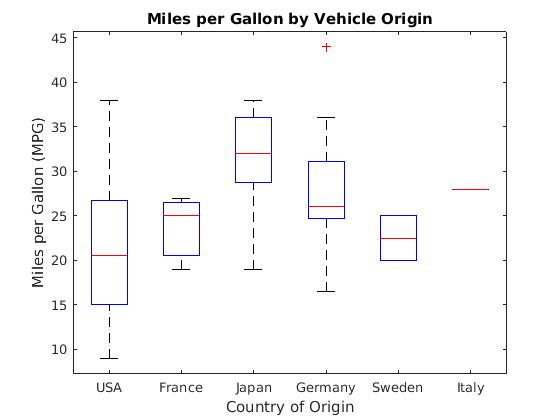
\includegraphics[width=.8\linewidth]{box2}
		\caption{Vertical multiple boxplots in Matlab}
		\label{fig:box2}
	\end{subfigure}
	\caption{Example Box Plots}
	\label{fig:figbox}
\end{figure}


\subsection{Random Charts}
In other to have the most diverse dataset, so as to achieve a robust model, we decided to pick 120 random images for each chart type  from Junior et al. \cite{junior2017archi} and Po-shen et al. \cite{lee2016viziometrix}. The line-charts, bar-charts and, scatter-plots were already labeled and were taken from Junior et al. work and the box-plots which we had to label, were taken from Po-shen et al. work since, the prior did not contain box-plots. The randomly picked chart images, were then added to the already created dataset for training and testing. Figure \ref{fig:random} shows sample images from the already created chart images from the paper of Po-shen et al. and Junior et al.

\begin{figure}[!htbp]
	\begin{subfigure}[b]{0.5\textwidth}
		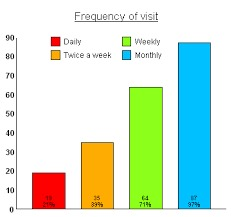
\includegraphics[width=\textwidth]{rand1}
		\caption{A bar-chart}
		\label{fig:rand1}
	\end{subfigure}
	%
	\begin{subfigure}[b]{0.5\textwidth}
		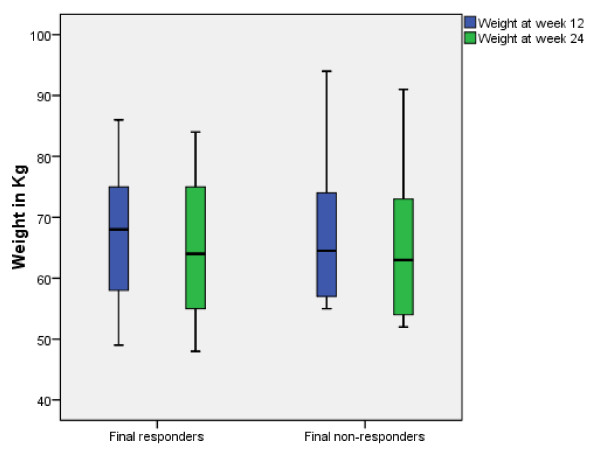
\includegraphics[width=\textwidth]{rand2}
		\caption{A box-plot}
		\label{fig:rand2}
	\end{subfigure}

	\begin{subfigure}[b]{0.5\textwidth}
		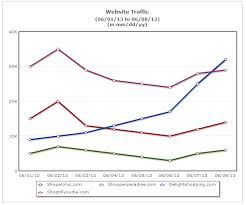
\includegraphics[width=\textwidth]{rand3}
		\caption{A line-chart}
		\label{fig:rand3}
	\end{subfigure}
	%
	\begin{subfigure}[b]{0.5\textwidth}
		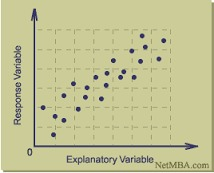
\includegraphics[width=\textwidth]{rand4}
		\caption{Scatter-plot}
		\label{fig:rand4}
	\end{subfigure}
	\caption{Example Chart images from Po-shen et al. and Junior et al.}
    \label{fig:random}
\end{figure}



\subsection{Training, Validation and Test set}
Figure ~\ref{fig:approach} summaries how our dataset was split into various activities. In machine learning, a model is an artifact created during the training phase, this model can be likened to a function that maps specific features to their respective labels, the model is trained with a portion of the dataset called the train set. As the model is trained, the validation set is used to decide and pick which metric out of hyper-parameters, early stopping and architecture considerations yields the best performance. This helps to adjust and optimise the model~\cite{validation}. Finally, the test-set in machine learning, is the other portion of the dataset which was not used during the training phase. The test-set checks how well the trained model performs on unseen data by giving an unbiased assessment of the model. For this work, the dataset is divided into train, validation and test set. The validation set is not shown in the figure since it forms part of the train data.

\begin{figure}[!htbp]
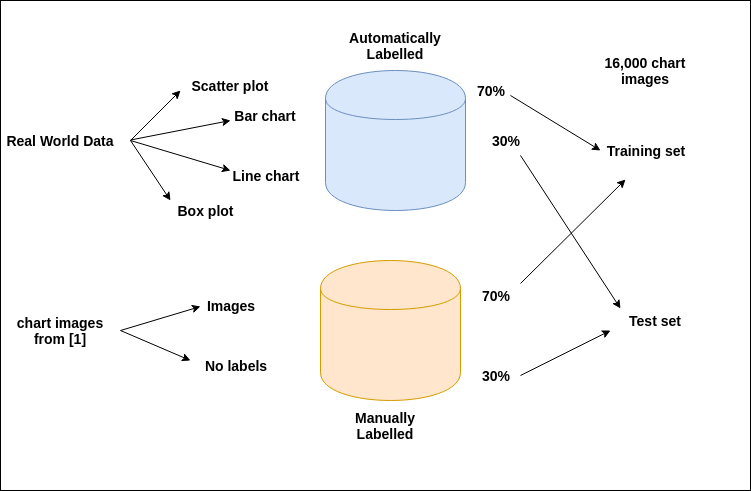
\includegraphics [scale=0.5] {approach}
\captionof{figure}{Steps involved in building the Classification model}
\label{fig:approach}
\end{figure}


\section{The Architecture}
As mentioned in previous sections, our model is trained with a CovNet. This architecture is inspired by the famous AlexNet CovNet architecture  \cite{krizhevsky2012imagenet}. The AlexNet architecture was used in the famous ImageNet LSVRC-2010 contest to classify 1.2 million into 1000 classes, the results obtained on the test-set had a top-5 error rate of 17.0\%, which was better than the previous state of the art. Our CovNet architecture just like the AlexNet architecture contains 8 learned layers, these 8 layers are made up of five Convolutional layers and 3 fully connected layers. A Relu is used after some Convolutional layers and fully connected layers. Another parameter employed in our architecture is a dropout, a dropout is applied in the first and second fully connected layers of our network and finally, max pooling is applied in some of the layers. A summary of our CovNet architecture used to train our model is shown in Figure~\ref{fig:archi}. The preprocessing steps, the parameters used, and why they were employed are explained into details in the rest of this chapter.

\begin{figure}
\centering
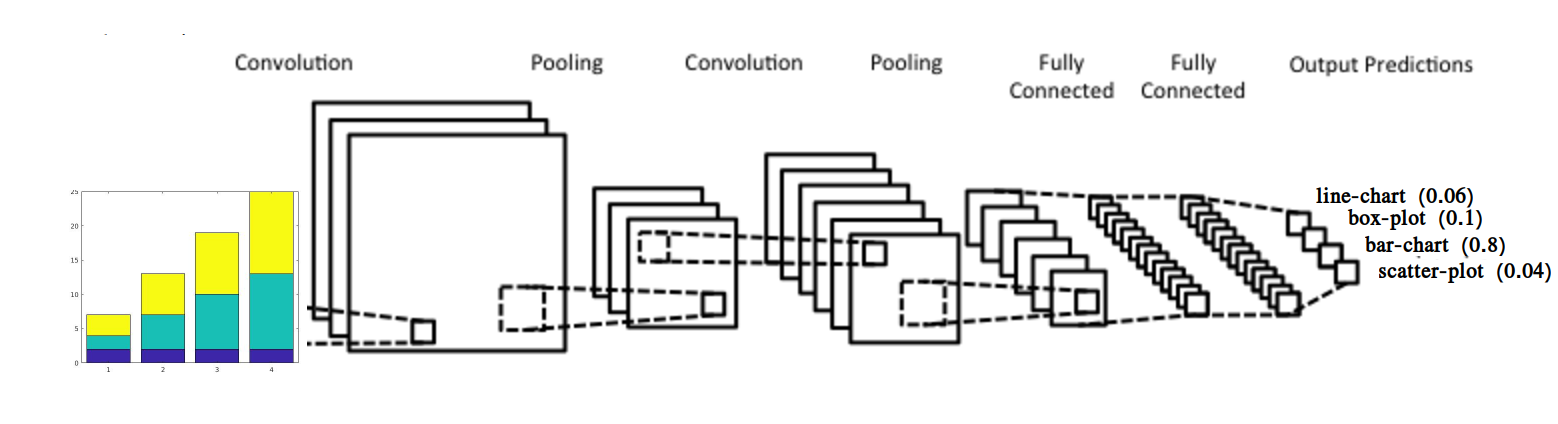
\includegraphics [scale=0.3] {architecture}
\captionof{figure}{Architecure of CovNet used to train our model}\label{fig:archi}
\end{figure}

\subsubsection{Convolutional Layer}
As mentioned above 5 of this layers are used in our architecture, and these are responsible for extracting the  features of the chart images. Our input image size used is 224 x 224 x 3  since its an RGB image, this is fed into our first Convolutional layer, this filters the image with a stride of 4 pixels. The second Convolutional layer takes as its input the output of the first Convolutional layer, between this two layers max-pooling is performed to reduce the size of the image. The third and fourth Convolutional layers, unlike the previous two have no max-pooling applied between them. The final Convolutional layer then takes as input the output of the previous layer and performs a max-pooling.

\subsection{Dropout}
A dropout was used in the first and second Fully connected layers in our architecture. We set dropout probability to 0.5 in our network, this means nodes are dropped out with a probability of 1-05 or or maintained at a probability of 0.5.


\subsection{Fully connected layers}
The last set of layers used are the Fully connected layers. 
The first layer takes as input the 1D feature vector generated by a flatten layer in our network. The flatten layer converts all our 2D arrays from our previous Convolutional layers into a 1D resultant vector. The output of this layer is then fed as input into the second fully connected layer. The output of the second layer is then fed into the last fully connected layer. The last layer in this set of 3 layers uses the softmax activation to give our output prediction. The output is a separate probability of our four classes and the choice with the highest probability is our chosen prediction. We used a sofmax activation as opposed to other activation functions because, it handles low invigoration
in images (say blurry charts) of your neural net with rather uniform distribution and to high invigoration in images (say large numbers, like sharp images) with prediction probabilities between 1 and 0.

\subsection{Preprocessing Techniques}
Archiving high performance by any machine learning technique is reliant on the quality and quantity of the data fed into the network.
Datasets must comprise of diverse data, this helps the network to generalise well during the testing phase. To help increase the quantity and also generate more diverse data we employ data augmenting techniques. The preprocessing techniques used in this thesis are described in the rest of this section.

\begin{itemize}
	\item  Image Resizing: The images have varying sizes and due to the presence of fully connected layer, we resize all the images to the size of 227 x 227. With this fixed image size processing in the dataset in batches is also possible.
	
	\item  Image Scaling: Object in the image can vary in size.
	
	
\end{itemize}


\begin{table}[!htbp]
	\centering \def\arraystretch{1.5} \small
	\label{table:2}
	\begin{adjustbox}{max width=1.1\textwidth,center}
		
		\begin{tabular}{|p{3cm}|p{3cm}|p{3cm}|p{3cm}|}
			\hline	
			Operation & Filter & Depth & Stride \\ \hline
			
			Conv1 + Relu  &  11 * 11  & 96  & 4 \\  \hline	 
			
			Max Pooling & 3 * 3  &  & 2 \\ \hline	   
			
			Conv2 + Relu & 5 * 5 & 256  &  \\ \hline	
			
			Max Pooling & 3 * 3 & & 2 \\ \hline
			
			Conv3 + Relu & 3 * 3 & 384 &  \\ \hline	
					
			
			Conv4 + Relu & 3 * 3  & 384  &  \\ \hline	
			
		    
		    Conv5 + Relu & 3 * 3  & 256 &  \\ \hline	
		    
		    Max Pooling & 3 * 3 & & 2 \\ \hline
		    
		    Dropout(rate 0.5) &  & & \\ \hline
		    
		    FC6 + Relu &  & & \\ \hline
		    
		    FC7 + Relu &  & & \\ \hline
		    
		    FC8 + Relu &  & & \\ \hline
		   
		\end{tabular}
	
	\end{adjustbox}

		\caption {The following table shows different layers, parameters and computation units used.}	
	
	
\end{table}












\chapter{Experiments}

\section{size of images was tried}


\chapter{Summary}

\bibliographystyle{unsrt}
\bibliography{sample}

\end{document}=====